\documentclass[10pt]{article}
\textwidth = 450pt
\headsep = 2pt
\headheight = 1pt
\oddsidemargin = 1pt

\usepackage{changepage}
\usepackage{fancyvrb}
\usepackage{graphicx}
\usepackage{amsmath}
\usepackage{capt-of}
\usepackage{amsfonts}
\usepackage{verbatim}
\usepackage{courier}
\usepackage{float}
\restylefloat{table}

%%%%%%%%%%%%%%%%%%% Code %%%%%%%%%%%%%%%%%%%%%%
\usepackage{color}
\usepackage[table]{xcolor} %adding background color to your tables
\usepackage{listings}% Allows you to present C++ syntax as it looks
\usepackage{listings} %enables inputing code set the settings below
\definecolor{dkgreen}{rgb}{0,0.45,0}
\definecolor{gray}{rgb}{0.2,0.5,0.5}
\definecolor{mauve}{rgb}{0.58,0,0.82}
%\definecolor{purple}{RGB}}{204, 45, 109}
\lstset{ %
language=C, % choose the language of the code
commentstyle=\color{dkgreen},
basicstyle=\footnotesize, % the size of the fonts that are used for the code
numbers=left, % where to put the line-numbers
numberstyle=\footnotesize, % the size of the fonts that are used for the line-numbers
stepnumber=1, % the step between two line-numbers. If it is 1 each line will be numbered
numbersep=5pt, % how far the line-numbers are from the code
backgroundcolor=\color{white}, % choose the background color. You must add \usepackage{color}
showspaces=false, % show spaces adding particular underscores
showstringspaces=false, % underline spaces within strings
showtabs=false, % show tabs within strings adding particular underscores
frame=single, % adds a frame around the code
tabsize=2, % sets default tabsize to 2 spaces
captionpos=b, % sets the caption-position to bottom
breaklines=true, % sets automatic line breaking
breakatwhitespace=false, % sets if automatic breaks should only happen at whitespace
keywordstyle=\color{purple}, % keyword style
numberstyle=\tiny\color{gray}, % the style that is used for the line-numbers
rulecolor=\color{black}, % if not set, the frame-color may be changed on
stringstyle=\color{blue}, % string literal style
escapeinside={\%*}{*)} % if you want to add a comment within your code
}
\DefineVerbatimEnvironment{code}{Verbatim}{fontsize=\small}
\DefineVerbatimEnvironment{example}{Verbatim}{fontsize=\small}
%%%%%%%%%%%%%%%%%%%%%%%%%%%%%%%%%%%%%%%%%%%%%%%%

\begin{document}
\title{Using Kinect to Evaluate Dance Performances\\ Third Year Group Project}
\author{Stylianos Venieris, Marcin Baginski, Theo Pavlakou, \\Zeping Xue, Yijie Ge \& Hesam Ipakchi  }
\date{\today}
\maketitle
\pagenumbering{gobble}
\newpage

\pagenumbering{arabic}
\setcounter{page}{1}
\section*{\center Abstract}

\section{Kinect \& NiTE Software Evaluation}
\noindent
To determine a method of evaluating the dance student, the limitations of the camera and the NiTE software must first be evaluated with respect to the criteria addressed below. To do this we use the UserViewer Application that comes as a sample with the NiTE software library with the camera elevated 75 cm above the ground, within the 60 cm to 180 cm range that is suggested by Microsoft for optimal tracking. 

\subsection{Camera Range}
\noindent 
To test for the camera's range, we lay a tape measure on the ground starting from directly below the camera up to 8 m away from the camera. We then use two subjects of different heights and body shapes to evaluate the performance of the camera and the software for tracking at different distances. The subject first starts within a few centimetres of the camera and slowly moves backwards until the camera calibrates and starts tracking and continues to do so until the tracking is lost. After this, the subject is required to start from the depths of the room, much further than the range of the camera, and to start walking slowly towards the camera, again taking a record of the following specifications. The results can be shown in Tables \ref{cam_range_180_away} to \ref{cam_range_150_toward}.
\\
\begin{table}[h]
\center
\begin{tabular}{ | l | c |}
\hline
Distance from Camera/cm & Description of Performance \\
\hline
60 & Identification of subject. Tracking. No skeleton.\\
120 & Skeleton fitted\\
410 & Tracking is lost\\
\hline
\end{tabular}
\caption{Subject moving away from camera. Subject height 180 cm.}
\label{cam_range_180_away}
\end{table}

\begin{table}[h]
\center
\begin{tabular}{ | l | c |}
\hline
Distance from Camera/cm & Description of Performance \\
\hline
100 & Identification of subject. Tracking. No skeleton.\\
120 & Skeleton fitted\\
410 & Tracking is lost\\
\hline
\end{tabular}
\caption{Subject moving towards camera. Subject height 180 cm.}
\label{cam_range_180_toward}
\end{table}

\begin{table}[h]
\center
\begin{tabular}{ | l | c |}
\hline
Distance from Camera/cm & Description of Performance \\
\hline
70 & Identification of subject. Tracking. No skeleton.\\
110 & Skeleton fitted\\
430 & Tracking is lost\\
\hline
\end{tabular}
\caption{Subject moving away camera. Subject height 150 cm.}
\label{cam_range_150_away}
\end{table}

\begin{table}[h]
\center
\begin{tabular}{ | l | c |}
\hline
Distance from Camera/cm & Description of Performance \\
\hline
50 & Identification of subject. Tracking. No skeleton.\\
110 & Skeleton fitted\\
430 & Tracking is lost\\
\hline
\end{tabular}
\caption{Subject moving towards camera. Subject height 150cm.}
\label{cam_range_150_toward}
\end{table}
\noindent
These results highlight the fact that the camera has a restricted field of view and therefore the number of people that each camera can support is limited. This will have to be further considered when finalising a design for the application. One thing to note is that, since  the optimum distance away from the camera, with respect to tracking, is in the range of 1.5m to 3.5m it would not be beneficial to have the camera(s) in the corners of the room. This would cause a huge amount of the already small range to be wasted due to the height of the room. 

\subsection{Effect of Varying Lighting Conditions}
\noindent
In order to evaulate the effect of varying lighting conditions on the tracking capabilities of the camera, we utilise a lux meter to determine the intensity of light in a room. The meter has been calibrated such that a complete darkness represents 0 lux. We then perform a series of tests to determine, if the varying lighting conditions have an effect on the tracking range of the camera. The table below presents the results of the tests:
\begin{table}[h]
\center
\begin{tabular}{ | l | c |}
\hline
Light intensity & Tracking range (starts - stops tracking) \\
\hline
4 lux & 120 cm - 420 cm\\
16 lux & 120 cm - 420 cm\\
44 lux & 120 cm - 420 cm\\
142 lux & 120 cm - 420 cm\\
176 lux & 120 cm - 420 cm\\
\hline
\end{tabular}
\caption{Tracking range in varying light intensity of the room}
\label{cam_range_varying_light}
\end{table}

\noindent
Since the skeleton is primarily fitted using the depth sensor of the RGB-D camera, the light intensity was expected to have little, if any, effect on the tracking range of the camera. Initially, we were expecting that the higher intensity of light might have a negative impact on the effectiveness of the IR depth sensor, however this has not been the case. It has been confirmed that varying light intensity, within bounds that we were able to achieve, have no effect on the range of the camera and its tracking capabilities.

\subsection{Obstruction in Range}
\noindent
To test for the possibility that obstructions could interfere with the fitting of the skeleton on the subject, we place a chair in various positions around the subject and in front of the subject. We then do the same with another person walking in the vicinity of the subject. This scenario is probably more relevant to the situations which may be encountered in a dance class room.  
\subsubsection{Chair}
\noindent Positioning the chair adjacent to the subject produces interesting results. When the chair is directly in front of the subject, the NiTE software tries to fit a skeleton to the chair as well as the person.
%% CHANGE
This can be seen in Figure \textbf{ADD FIGURE}. Putting the chair on the head of the subject and at the waist does not give this result, but instead the proportion of the skeleton that is created by the software is quite distorted
%% CHANGE
(see Figure \textbf{ADD FIGURE}). 
%% CHANGE
% Not finished. It seems that this section is quite a hand waving description of the experiment because we probably could have been more thorough.  
\subsubsection{Person}
\noindent
In this experiment the second person walks within different ranges of the camera and the initial subject. Interestingly enough, even at quite fast speeds of movement, the camera can calibrate and track both people quite quickly. This will most probably not be a limitation when creating the software. 
\subsection{Velocity of Movement}
Another important criterion regarding the performance of both the Kinect camera and the NiTE software package is the accuracy and responsiveness of the skeleton fitting. Our evaluation procedure consists of the recording of a predefined movement which would provide us with the subject's velocity information and would allow us to estimate how accurately the fitted skeleton is able to follow the actual move, by calculating the error between the perceived and the actual movement. In particular, we would record a slower and a faster versions of the same movement and compare the corresponding errors.

The subject's reference movement was determined to be a $180^o$ degrees right arm move starting from a vertical position with the hand facing the ceiling and following an arc. The testing procedure includes the modification of the \texttt{UserViewer} sample program in order to record twice the predefined movement as performed by the subject at high and low speeds. 

By capturing the recorded passage with a Desktop camera at a rate of 24 frames per second(fps), we are able to extract individual frames from the recorded videos. At this point, we define a starting and an ending point of the subject's right arm and select the frames that more accurately correspond to these positions. After following this procedure for both recordings, we end up with 3 frames from the fast and 16 from the slow version. The starting and ending position frames for the slow and the fast versions are shown below on Figure \ref{start_pos}. The substantial deviation between the shoulder-elbow vertex of the skeleton and the arm indicate the important increased error when the subject performs a fast move.

\begin{figure}[h]
\center
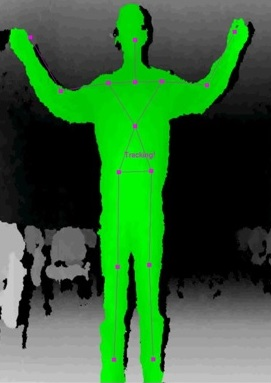
\includegraphics[scale=0.5]{SlowStart.jpg} 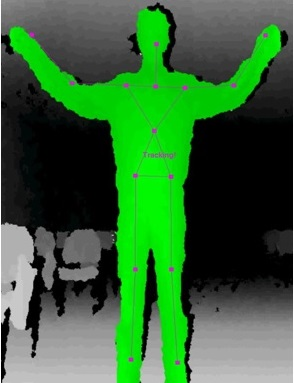
\includegraphics[scale=0.5]{FastStart.jpg}
\caption{Slow and fast recordings starting position.}
\label{start_pos}
\end{figure}

\begin{figure}
\center
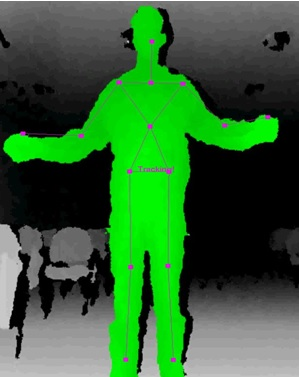
\includegraphics[scale=0.5]{SlowEnd.jpg} 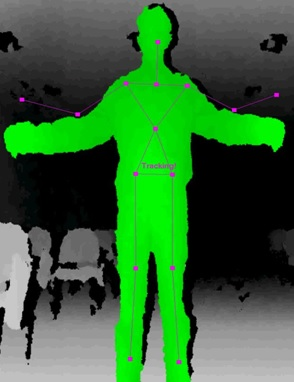
\includegraphics[scale=0.5]{FastEnd.jpg}
\caption{Slow and fast recordings ending position, with substantial error in the fast version's skeleton fitting.}
\end{figure}


\noindent A summary of the number of frames and the time between the starting and ending arm position for each  is shown below.

\begin{table}[H]
\center
\begin{tabular}{| c | c | c |}
\hline
Movement Speed & Number of Frames & Movement Duration/sec\\
\hline
Fast & 3 & 0.083\\
Slow & 16 & 0.670\\
\hline
\end{tabular}
\caption{Movement duration for fast and slow versions, recorded at 24 fps.}
\end{table}

The next step of the responsiveness evaluation is the estimation of the arm's actual starting and ending positions as well as its perceived position as defined by the fitted skeleton. As the arm follows an arc-shaped movement, we focus on measuring the angle between the subject's elbow and shoulder, with the shoulder  defined as the reference, and finding an estimate of the skeleton fitting error by comparing the actual angle and the angle of the vertex between the two joints with respect to the shoulder joint. Although both the actual and perceived starting positions are the same, the ending positions are different and result in errors in the subject's tracking. The angle measurements can be seen below in Table \ref{angle}.

\begin{table}[H]
\center
\begin{tabular}{| c | c | c | c |}
\hline
Movement Speed & Starting Angle/deg & Perceived Ending Angle/deg & Actual Ending Angle/deg\\
\hline
Fast & $3.5^o$ & $-30.5^o$ & $-55.3^o$\\
Slow & $4.4^o$ & $-49.2^o$ & $-64.0^o$\\
\hline
\end{tabular}
\caption{Perceived and actual starting and ending angles of the subject's arm.}
\label{angle}
\end{table}

The final step involved the estimation of the actual and perceived angular velocities based on the already obtained data and the calculation of the error as a consequence to the difference between them. By using the following formula, we estimate the angular velocities and the errors for both the slow and the fast recordings.
\begin{equation}
\omega = RotationalDisplacement * MovementDuration
\end{equation}

\noindent where \[RotationalDisplacement = EndingAngle - StartingAngle\]
and  $\omega$ stands for the angular velocity

\noindent The angular velocities and the corresponding errors for both the slow and the fast recordings are presented on the following table.

\begin{table}[H]
\center
\begin{tabular}{| c | c | c | c |}
\hline
Movement Speed & Perceived Angular Velocity/$^o/s$ & Actual Angular Velocity/$^o/s$ & Error/\% \\
\hline
Fast & $-408.0$ & $-705.0$ & $42.12\%$ \\
Slow & $-67.2$ & $-89.4$ & $24.8\%$ \\
\hline
\end{tabular}
\caption{Perceived and actual angular velocities and percentage errors.}
\end{table}

As a result, ... % CHANGE

\subsection{Camera Angle Relative to Subject}


\subsection{Multiple People}
\noindent
In order to discover how many subject can be tracked by a single camera, we test with multiple people standing in front of it. The standard we have for a subject being fully visible is that the software \texttt{UserViewer} can identify all joints. Skeleton missing head or leg joints are invalid for our project. Improper results can be viewed in software as missing joints wrong identifications of skeleton for a subject, for example, one subject has part of its body skeleton actually belong to another subject. The test result is that 5 subjects is the maximum the camera and software can detect. Subjects are required to be in two rows, two in the front and three in the back so that they do not cover each other.\\
 
\begin{figure}[hbtp]
\centering
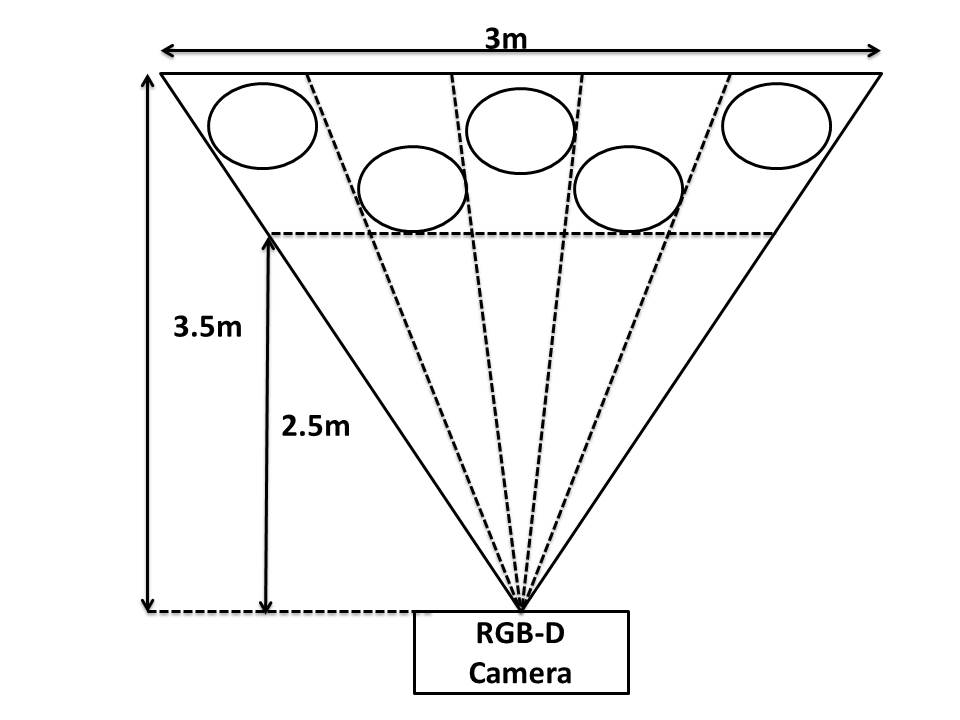
\includegraphics[scale=1]{multi_people1.jpg}
\caption{how subjects are placed}
\end{figure}
 
\begin{figure}[hbtp]
\centering
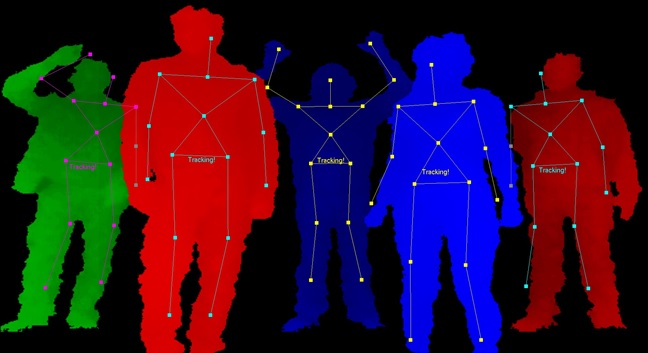
\includegraphics[scale=1]{multi_people2.jpg}
\caption{5 subjects tracked}
\end{figure}
 
As mentioned before, a subject needs to be 2.5 to 4 metres away from the camera to be fully visible. After splitting up the area for 5 subjects, each one has less than 1 metre square which is not enough for dance. 3 is an optimal number of subjects for a single camera to track.\\


\subsection{Multiple Cameras}
\noindent
There may be a requirement to use multiple cameras for the finalised product so testing to see whether a setup using more than one camera has an effect on the performance of the hardware is something that must be considered. Research has suggested that using more than one camera with an overlapping view between them can lead to depth images that contain `holes' in them
%% CHANGE
\textbf{ADD REFERENCE TO SHAKE\_N\_SENSE}. To test whether this will be a problem we use the following setup 
%% CHANGE: Add sketch of setup for testing of two cameras
\textbf{ADD FIGURE}. In this setup the two cameras have overlapping views and also are completely facing each other, which means there will be interference from one camera to the next. 
\\\\
\noindent
The subjects stand and move in front of the camera at a distance of at least 2m from each camera. No noticeable interference is present when the subjects are in front of the IR light source of each of the cameras so that the camera opposite cannot detect the IR pattern created by it. But when there is no one in front of the camera, we can see that there is indeed a large `hole' that can be seen in the depth image due to the IR pattern of camera opposite it. 
%% CHANGE
\textbf{ADD FIGURE}
This is a possible configuration for the dance class and as long as there are people in front of both cameras, blocking their IR stream to stop interference, it is highly plausible as the experiments show. On all occasions the subjects are tracked by both cameras with no perceived deterioration in the performance. 

\subsection{Analysis of Results}
\clearpage

\section*{Appendix}
\subsection*{Some Code}
\begin{lstlisting}
int main()
{
	// your code
	x = 5;
}

\end{lstlisting}
\end{document}
